\section{Ablation and check register}
\label{app:ablation}

Table~\ref{tab:ablation-register} records what was isolated, what was merely compared,
and what was not isolated. A tick in the first column means the factor was removed or
replaced while everything else was held fixed; a dash means the evidence is a comparison
of complete pipelines rather than an ablation of one component.

\begin{longtable}{p{0.04\linewidth}p{0.18\linewidth}p{0.19\linewidth}p{0.27\linewidth}p{0.16\linewidth}}
\caption{Ablation register. Every row names the factor, the levels actually run, the
table or section that reports the result, and the verdict. The last two rows are
deliberate gaps and are not claimed as isolated effects in the text.}
\label{tab:ablation-register}\\
\toprule
Isol. & Factor & Levels run & Reported in & Verdict \\
\midrule
\endfirsthead
\toprule
Isol. & Factor & Levels run & Reported in & Verdict \\
\midrule
\endhead
\bottomrule
\endfoot
\multicolumn{5}{l}{\emph{Problem 1}}\\
yes & Zero-parameter segmentation & constant, midpoint, blind thirds & Table~\ref{tab:appL-p1a} & none beats the rule \\
yes & Feature set $\times$ clustering & raw vs head frame; Ward vs constrained & Table~\ref{tab:ablation} & features help, constraint helps \\
yes & Decoder & Ward, oracle $K$, peak rule, bi-TCN & Table~\ref{tab:appL-p1a} & peak rule and bi-TCN trade ARI for boundary F1 \\
yes & Reliability route & calibrated, geometric, fused & Table~\ref{tab:rel} & fused is the deployed route \\
yes & Detector width & V1--V8, 3 seeds each & Table~\ref{tab:p1b-arms} & V8 clears both gates \\
yes & Leave-one-task-class-out & 26 classes & Table~\ref{tab:loto} & gap to in-sample reference reported \\
yes & Representative point & palm full, four palm LOO, tips full, five tip LOO & Table~\ref{tab:p1-loo} & palm does not depend on any one MCP \\
yes & Representative point, retrained & wrist, palm, tips; both learners refit & Table~\ref{tab:p1-anchor} & the anchor moves the result by less than the seed spread \\
yes & Stage thresholds & five thresholds at $0.8\times$, $1.0\times$, $1.2\times$ & Table~\ref{tab:p1-thr} & $v_{lo}$ moves 6.35~pp; labels otherwise stable \\
\midrule
\multicolumn{5}{l}{\emph{Problem 2}}\\
yes & Predictor ladder & hold, CV, CA, ridge, GRU, quantile & Tables~\ref{tab:p2grid} and~\ref{tab:appL-p2} & ridge wins short, quantile wins at every official length \\
yes & Mask length & \slotMaskA, \slotMaskB, \slotMaskC, \slotMaskD{} s & Table~\ref{tab:p2grid} & all four reported; no interpolation between them \\
yes & Training for missing input & clean, LOCF, interpolation & Section~\ref{sec:p2res} & null: under two millimetres \\
yes & Reliability as training weight & hard filter, soft weight, neither & Section~\ref{sec:p2res} & null: interval crosses zero \\
yes & Interval construction & split conformal, marginal coverage & Table~\ref{tab:intervals} & coverage reported per mask \\
yes & Cost rule & fixed short, fixed long, reactive, priced & Table~\ref{tab:econ} & priced optimum is interior \\
yes & Context length & 5, 10, 20, 40 frames at $L=1.0$~s & Table~\ref{tab:ctx-ablation} & flat: 6.25--6.32~cm, no gain from more context \\
yes & Ridge feature subset & full, no acceleration, relative only, no horizon columns & Table~\ref{tab:feature-ablation} & null: 6.298~cm in every variant \\
\midrule
\multicolumn{5}{l}{\emph{Problem 3}}\\
yes & Policy ladder & EDF, slack, risk, rollout, oracle & Table~\ref{tab:p3nom} and Figure~\ref{fig:policy} & the rule buys the points; oracle is the ceiling \\
yes & Mapping sensitivity & five $(\alpha,\beta)$ maps & Table~\ref{tab:alpha-sweep} & the ordering survives every map \\
yes & Paid review & 270 cells, 15 policies & Appendix~\ref{app:scorecard} & nothing clears one point \\
yes & Reservation learner & 13 quantile actions, 15 seeds & Appendix~\ref{app:secondround} & no gain over the grid corner \\
yes & Reservation level & $q\in[0.30,0.90]$ & Figure~\ref{fig:phase} & flat in $q$, steep in $\alpha$ \\
yes & Rule knobs & 8 one-at-a-time moves & Table~\ref{tab:p3-sens} & OAT, local dependence only \\
yes & Rule knobs & $2^7$ full factorial, 128 corners & Table~\ref{tab:p3-factorial} & frozen policy above every corner; $k$ and $q_{sl}$ inert \\
yes & Rule knobs & $3^5$ three-level design, 243 cells & Table~\ref{tab:p3-threelevel} & curvature is real and negative; no pair restores the loss \\
\end{longtable}

\begin{table}[H]
\centering
\caption{Context-length ablation for the ridge predictor at $L=1.0$~s. Only the number of
context frames changes; records, mask length, penalty and feature map are fixed. Test is
read once per row.}
\label{tab:ctx-ablation}
\footnotesize
\begin{tabular}{rrrr}
\toprule
Context (frames) & Training windows & Test windows & Three-dimensional RMSE (cm) \\
\midrule
5 & 2,909 & 745 & 6.252 \\
10 & 2,884 & 738 & 6.298 \\
20 & 2,817 & 721 & 6.323 \\
40 & 2,704 & 692 & 6.307 \\
\bottomrule
\end{tabular}
\end{table}

\begin{table}[H]
\centering
\caption{Feature-subset ablation for the ridge predictor at $L=1.0$~s and context 10.
Only the feature map changes; records, windows, mask length and penalty are fixed.}
\label{tab:feature-ablation}
\scriptsize
\begin{tabular}{p{0.42\linewidth}rrr}
\toprule
Feature map & Features & Test windows & Three-dimensional RMSE (cm) \\
\midrule
Full (relative + velocity + acceleration + horizon) & 38 & 738 & 6.298 \\
No acceleration & 35 & 738 & 6.298 \\
Relative only & 32 & 738 & 6.298 \\
Full without horizon columns & 36 & 738 & 6.298 \\
\bottomrule
\end{tabular}
\end{table}

The two P3 tables answer different questions. The one-at-a-time table measures local
dependence around the frozen policy; the full factorial crosses all seven knobs at two
levels and therefore also exposes interactions. The frozen policy sits above all 128
corners in both cases, and the corner range is \slotPFactRangeSTwo{} and
\slotPFactRangeSThree{} points, so the selected point is not an artefact of a lucky
one-dimensional move. Two knobs are structurally inactive under the selected rules: the
slack coefficient $k$ and the slack quantile $q_{sl}$ change nothing once the rule is
``fix'' or ``absorb'', which is why their main effects are exactly zero. Neither table
re-selects the policy; selection remains the joint search on validation described in
Section~\ref{sec:p3model}.

A two-level design cannot separate curvature from interaction, so the five knobs that do
act are crossed again at three levels, with the frozen value as the middle level
(Table~\ref{tab:p3-threelevel}). The frozen policy is again the best or near-best cell: it
sits above \slotPThreeAboveSTwo{} of the 243 cells in S\slotCaseTwo{} and above
\slotPThreeAboveSThree{} in S\slotCaseThree{}, over a total range of
\slotPThreeRangeSTwo{} and \slotPThreeRangeSThree{} points. The coded model recovers only
$R^2=\slotPThreeRTwoSTwo$ and \slotPThreeRTwoSThree{}, which is itself the finding: most of
the variation is curvature and noise rather than a clean linear response. Every curvature
term is negative except two small positive ones in S3, so moving a knob away from the
frozen value loses more than a linear reading would predict, and the strongest pair is
$gate\times late\_tol$ at \slotPThreeInterSTwo{} points in S\slotCaseTwo{} and
\slotPThreeInterSThree{} in S\slotCaseThree{}.

The representative point is tested the same way in Table~\ref{tab:p1-anchor}: instead of
re-measuring a metric under a moved keypoint, both learners are refitted from scratch on a
state tensor rebuilt around the wrist, the palm centroid and the fingertip centroid. Part~I
turned out not to be bit-reproducible: two runs on a bit-identical input differ by more than
a point of ARI, so every anchor is run five times and reported as a mean with its spread,
and the anchor contrast is compared against that spread rather than against zero. At five
runs the fingertip advantage over the wrist, \slotPAnchorTipsMinusWrist{} points with a
standard error of \slotPAnchorSE{} points, does not clear that spread, so the earlier claim
that the anchor mattered for the segmenter is withdrawn; what survives is the disagreement in
direction, with the detector still losing most of its average precision at the fingertip
anchor. No single anchor is best for the whole chain, so the paper declares one per part
instead of claiming a global optimum.

\begin{table}[H]
\centering
\caption{Leave-one-keypoint-out for the representative point. Each row removes one keypoint from the palm set or from the fingertip set and recomputes the same within-record rigidity on all 66,070 frames. A near-zero change means the choice does not rest on any single joint.}
\label{tab:p1-loo}
\scriptsize
\begin{tabular}{lrrrr}
\toprule
Candidate & Points & Rigidity (cm) & Jitter ratio & $\Delta$ rigidity (cm) \\
\midrule
wrist kp0 & 1 & 0.00005 & 0.1389 & +3.73e-05 \\
palm full & 5 & 0.00001 & 0.1382 & +0.00e+00 \\
tips full & 5 & 1.53823 & 0.1428 & +1.54e+00 \\
palm minus kp5 & 4 & 0.00002 & 0.1386 & +3.22e-06 \\
palm minus kp9 & 4 & 0.00002 & 0.1383 & +3.65e-06 \\
palm minus kp13 & 4 & 0.00002 & 0.1379 & +2.14e-06 \\
palm minus kp17 & 4 & 0.00001 & 0.1376 & -1.19e-07 \\
tips minus kp4 & 4 & 1.81347 & 0.1441 & +1.81e+00 \\
tips minus kp8 & 4 & 1.53952 & 0.1441 & +1.54e+00 \\
tips minus kp12 & 4 & 1.43624 & 0.1434 & +1.44e+00 \\
tips minus kp16 & 4 & 1.45425 & 0.1424 & +1.45e+00 \\
tips minus kp20 & 4 & 1.58826 & 0.1422 & +1.59e+00 \\
\bottomrule
\end{tabular}
\end{table}

\begin{table}[H]
\centering
\caption{Stage-threshold sweep. Each row moves one threshold to $0.8\times$ or $1.2\times$ its default and relabels all 66,070 frames with everything else fixed. The last two columns are the largest change in any stage's share of frames and in the mean segment length, relative to the default.}
\label{tab:p1-thr}
\footnotesize
\begin{tabular}{lrrrrr}
\toprule
Threshold & Default & $0.8\times$ & $1.2\times$ & Max share shift (pp) & Segment length change \\
\midrule
$v_{\mathrm{hi}}$ & 0.1 & 0.08 & 0.12 & 2.18 & +0.038 \\
$v_{\mathrm{lo}}$ & 0.05 & 0.04 & 0.06 & 6.35 & +0.325 \\
$a_{\mathrm{grasp}}$ & 0.15 & 0.12 & 0.18 & 1.29 & +0.000 \\
$t_{\mathrm{arr}}$ & 0.8 & 0.64 & 0.96 & 0.71 & +0.000 \\
$a_{\mathrm{cl}}$ & 0.55 & 0.44 & 0.66 & 4.88 & +0.000 \\
\bottomrule
\end{tabular}
\par\smallskip\footnotesize Default share of frames: reach 65.63, pick 7.15, place 4.70, transport 17.30, arrange 5.22. Mean segment length at the default is 60.15 frames.
\end{table}

\begin{table}[H]
\centering
\caption{The representative point, retrained rather than re-measured. Every row re-runs the same learners from scratch on a state tensor built around a different anchor: identical seeds, identical record-level split, identical hyper-parameters, identical decoding grid, test scored once. Part I is the segmenter (3 seeds, 40 epochs) and is reported as mean $\pm$ sd over repeated runs, because the same input does not reproduce the same run; Part II is the frozen production detector (V8, 3 seeds, 18 epochs).}
\label{tab:p1-anchor}
\scriptsize
\begin{tabular}{lrrrrrr}
\toprule
Anchor & \multicolumn{3}{c}{Part I segmenter} & \multicolumn{3}{c}{Part II detector} \\
\cmidrule(lr){2-4}\cmidrule(lr){5-7}
 & ARI (mean $\pm$ sd) & runs & $\Delta$ARI (pp) & AP & AUC & Worst env. \\
\midrule
wrist & 0.5278 $\pm$ 0.0313 & 5 & +0.00 & 0.1493 & 0.8271 & 0.7777 \\
palm & 0.5440 $\pm$ 0.0355 & 5 & +1.62 & 0.1236 & 0.8075 & 0.7393 \\
tips & 0.5613 $\pm$ 0.0292 & 5 & +3.35 & 0.0819 & 0.8099 & 0.7519 \\
\bottomrule
\end{tabular}
\par\smallskip\footnotesize Wrist is the anchor the main pipeline uses, so its row is the reference. The two learners disagree: tips is the best anchor for the segmenter and the worst for the detector, so the choice of representative point is load-bearing and must be declared per part rather than fixed once for the paper. The pooled within-anchor sd is 0.0320 ARI; tips minus wrist is +3.35 points with a standard error of 1.92 points, which falls inside the noise.
\end{table}

\begin{table}[H]
\centering
\caption{One-at-a-time sensitivity of the frozen Part III policy. Every other sub-parameter is held at its selected value; each row moves one knob to two nearby values and re-runs all 30 seeds on five mappings. $\Delta$ is the weighted on-time rate in percentage points against the frozen row.}
\label{tab:p3-sens}
\footnotesize
\begin{tabular}{llrrr}
\toprule
Case & Knob moved & Values & $\Delta$ range (pt) & Cost ratio \\
\midrule
S2 & reservation quantile $q$ & 0.30, 0.60 & [-0.89, +0.22] & [0.994, 1.004] \\
S2 & release gate & 0.55, 0.95 & [-2.78, -1.33] & [0.981, 0.998] \\
S2 & lateness tolerance (s) & 4.0, 20.0 & [-2.28, -1.08] & [0.979, 1.000] \\
S2 & selector mix & 0.30, 0.90 & [-2.11, -0.25] & [0.996, 0.999] \\
S2 & blocking weight & 0.25, 0.50 & [-0.08, -0.08] & [1.000, 1.000] \\
S2 & slack coefficient $k$ & 0.40, 0.80 & [+0.00, +0.00] & [1.000, 1.000] \\
S2 & slack quantile & 0.40, 0.80 & [+0.00, +0.00] & [1.000, 1.000] \\
\midrule
S3 & reservation quantile $q$ & 0.20, 0.45 & [-1.15, +0.12] & [0.996, 1.006] \\
S3 & release gate & 0.15, 0.55 & [-0.02, +0.00] & [0.999, 1.000] \\
S3 & lateness tolerance (s) & 12.0, 28.0 & [-2.52, -1.02] & [0.996, 1.002] \\
S3 & selector mix & 0.00, 0.45 & [-0.23, -0.10] & [0.998, 1.000] \\
S3 & blocking weight & 0.00, 0.50 & [+0.04, +0.12] & [1.000, 1.000] \\
S3 & slack coefficient $k$ & 0.40, 0.80 & [+0.00, +0.00] & [1.000, 1.000] \\
S3 & slack quantile & 0.40, 0.80 & [+0.00, +0.00] & [1.000, 1.000] \\
S3 & review hurdle $\tau$ & 0.01, 0.05 & [+0.00, +0.00] & [1.000, 1.000] \\
\bottomrule
\end{tabular}
\end{table}


\begin{table}[H]
\centering
\caption{Two-level full factorial over the seven rule knobs ($2^7=128$ corners per case, 30 seeds, five mappings). The upper panel locates the frozen policy inside the corner distribution; the lower panel is the main effect of each knob averaged over the other six. Zero means the knob is structurally inactive under the selected rule.}
\label{tab:p3-factorial}
\scriptsize
\begin{tabular}{lrrrrrr}
\toprule
Case & Frozen & Corner min & Corner med. & Corner max & Range (pp) & Frozen pct. \\
\midrule
S2 & 0.8486 & 0.7883 & 0.8061 & 0.8406 & 5.22 & 100 \\
S3 & 0.8056 & 0.7392 & 0.7873 & 0.8017 & 6.25 & 100 \\
\midrule
\multicolumn{7}{l}{\emph{Main effect on the weighted on-time rate (pp)}}\\
Case & $q_{hi}$ & gate & late tol. & mix & gam & $k$, $q_{sl}$ \\
\midrule
S2 & -1.12 & -0.11 & +0.99 & -0.80 & +0.04 & 0.00 \\
S3 & -1.22 & +0.61 & +4.46 & +0.07 & -0.02 & 0.00 \\
\bottomrule
\end{tabular}
\end{table}

\begin{table}[H]
\centering
\caption{Three-level design on the five knobs that actually act ($3^5=243$ cells per case, 30 seeds, five mappings). The middle level of each knob is its frozen value. Upper panel: where the frozen policy sits. Lower panel: least-squares coefficients of a coded linear model with all ten pairwise products, in on-time points; the curvature column is the pure quadratic term read off the centre cell.}
\label{tab:p3-threelevel}
\scriptsize
\begin{tabular}{lrrrrrr}
\toprule
Case & Frozen & Cell min & Cell max & Range (pp) & Above frozen & Model $R^2$ \\
\midrule
S2 & 0.8486 & 0.7883 & 0.8508 & 6.25 & 6/243 & 0.419 \\
S3 & 0.8056 & 0.7388 & 0.8106 & 7.19 & 36/243 & 0.631 \\
\midrule
\multicolumn{7}{l}{\emph{Main effects and curvature (pp)}}\\
\midrule
Case & $q\_hi$ & $gate$ & $late\_tol$ & $mix$ & $gam$ \\
\midrule
S2 main & -0.55 & -0.18 & +0.54 & -0.57 & +0.01 \\
S2 curv & -0.36 & -2.10 & -1.67 & -1.19 & -0.04 \\
S3 main & -0.57 & +0.21 & +2.24 & +0.04 & +0.01 \\
S3 curv & -0.51 & +0.02 & -3.16 & -0.05 & +0.08 \\
\midrule
\multicolumn{7}{l}{\emph{Pairwise interactions (pp); only terms above $0.05$ in either case are listed}}\\
\midrule
Case & $q\_hi\times gate$ & $q\_hi\times late\_tol$ & $q\_hi\times mix$ & $q\_hi\times gam$ & $gate\times late\_tol$ \\
\midrule
S2 & +0.08 & +0.07 & -0.06 & +0.01 & -0.82 \\
S3 & -0.10 & +0.02 & -0.02 & -0.01 & -0.26 \\
\bottomrule
\end{tabular}
\par\smallskip\footnotesize The centre cell is not exactly the frozen policy for S2, because the frozen mixing weight sits at the lower end of the three-level range; the frozen policy is therefore run as its own candidate and every delta is measured against it.
\end{table}


\subsection{Tables moved out of the body}

\begin{table}[htbp]
\centering
\caption{The eleven measures the statement names, on the nominal mapping, mean over \slotNSeeds{} official seeds with one sampler and one seed set for every row. Tardiness, overrun, idle and elapsed are in seconds; censored counts trials that end with a job still running at the horizon; invalid is the number of protocol violations. S\slotCaseOne{} saturates for every policy and is reported in Appendix~\ref{app:scorecard}.}
\label{tab:p3score}
\scriptsize
\setlength{\tabcolsep}{3.0pt}
\begin{tabular}{lrrrrrrrrrrr}
\toprule
Policy & on-time & completion & tardiness & cost & overrun & idle & reviews & elapsed & censor & done & invalid \\
\midrule
\multicolumn{12}{l}{\emph{S\slotCaseTwo}}\\
Duration-aware reference (p known) & 0.860 & 0.868 & 95.9 & 30.0 & 20.4 & 7.2 & 0.00 & 98.0 & 0.53 & 10.20 & 0 \\
Risk fusion & 0.856 & 0.883 & 87.1 & 28.7 & 20.0 & 6.8 & 0.00 & 97.3 & 0.30 & 9.77 & 0 \\
Capacity-aware slack (incumbent) & 0.815 & 0.867 & 77.4 & 28.7 & 22.7 & 6.8 & 0.00 & 96.8 & 0.23 & 10.03 & 0 \\
Rollout lookahead & 0.736 & 0.846 & 268.4 & 29.2 & 16.3 & 8.5 & 0.00 & 94.5 & 0.20 & 10.37 & 0 \\
Slack with fused predictor & 0.796 & 0.867 & 81.5 & 29.0 & 22.6 & 6.0 & 0.00 & 97.4 & 0.30 & 10.10 & 0 \\
Earliest due date (statement reference) & 0.562 & 0.840 & 65.0 & 29.0 & 22.8 & 7.3 & 0.00 & 98.4 & 0.40 & 9.93 & 0 \\
Earliest due date, fused predictor & 0.574 & 0.842 & 60.6 & 28.8 & 22.9 & 6.7 & 0.00 & 97.9 & 0.37 & 9.93 & 0 \\
Adaptive-quantile reservation (ours) & 0.872 & 0.899 & 96.5 & 28.6 & 30.8 & 3.5 & 0.00 & 96.3 & 0.20 & 10.43 & 0 \\
\midrule
\multicolumn{12}{l}{\emph{S\slotCaseThree}}\\
Duration-aware reference (p known) & 0.815 & 0.846 & 182.0 & 37.1 & 25.6 & 10.2 & 0.00 & 120.4 & 0.13 & 13.30 & 0 \\
Risk fusion & 0.744 & 0.831 & 177.7 & 35.1 & 29.6 & 7.4 & 0.07 & 118.9 & 0.07 & 12.57 & 0 \\
Capacity-aware slack (incumbent) & 0.741 & 0.825 & 180.2 & 34.7 & 30.7 & 9.1 & 0.00 & 120.3 & 0.07 & 12.43 & 0 \\
Rollout lookahead & 0.761 & 0.835 & 285.2 & 35.3 & 25.4 & 9.3 & 0.00 & 116.8 & 0.07 & 12.63 & 0 \\
Slack with fused predictor & 0.734 & 0.834 & 167.8 & 35.2 & 30.1 & 8.0 & 0.00 & 120.4 & 0.13 & 12.53 & 0 \\
Earliest due date (statement reference) & 0.522 & 0.822 & 158.3 & 36.2 & 29.0 & 9.3 & 0.00 & 122.1 & 0.23 & 12.80 & 0 \\
Earliest due date, fused predictor & 0.523 & 0.819 & 154.1 & 36.2 & 28.5 & 8.5 & 0.00 & 121.5 & 0.30 & 12.73 & 0 \\
Adaptive-quantile reservation (ours) & 0.821 & 0.881 & 168.5 & 34.9 & 41.3 & 3.3 & 0.00 & 117.8 & 0.03 & 13.10 & 0 \\
\midrule
\bottomrule
\end{tabular}
\end{table}


\begin{table}[htbp]
\centering
\caption{$2\times2$ ablation of feature set against clustering method (ARI / frame
F1). The interaction, not either factor, carries the gain.}
\label{tab:ablation}
\footnotesize
\begin{tabular}{llrr}
\toprule
Features & Method & ARI & Frame F1 \\
\midrule
Raw coordinates & $K$-means & \slotPAblKRawARI & \slotPAblKRawFOne \\
Raw coordinates & Ward & \slotPAblWRawARI & \slotPAblWRawFOne \\
Head frame & $K$-means & \slotPAblKHeadARI & \slotPAblKHeadFOne \\
Head frame & Ward & \slotPAblWHeadARI & \slotPAblWHeadFOne \\
\bottomrule
\end{tabular}
\end{table}

\begin{table}[htbp]
\centering
\caption{Competing partition families on the held-out records. Means over the same
records as Table~\ref{tab:seg}; all rows are below the reported baseline except the
last, which fails model selection.}
\label{tab:negative}
\footnotesize
\begin{tabular}{lr}
\toprule
Method & Mean ARI \\
\midrule
Hidden Markov model & \slotPSegHMMARI \\
Hidden Markov model, true count & \slotPSegHMMOracleARI \\
Autoencoder + hidden Markov model & \slotPSegAEHMMARI \\
Multi-scale Ward & \slotPSegWardMSARI \\
Autoencoder + Ward & \slotPSegAEWardARI \\
Constrained Ward, widened cap & \slotPSegWardKTwoFiveARI \\
\bottomrule
\end{tabular}
\end{table}

\begin{table}[htbp]
\centering
\caption{Per-environment reliability. The same fitted weight is applied to both
environments without recalibration.}
\label{tab:env}
\footnotesize
\begin{tabular}{lrrr}
\toprule
Environment & Frames & Positives & AUC \\
\midrule
\texttt{\slotPEnvOneName} & \slotPEnvOneN & \slotPEnvOnePos & \slotPEnvOneAUC \\
\texttt{\slotPEnvTwoName} & \slotPEnvTwoN & \slotPEnvTwoPos & \slotPEnvTwoAUC \\
\bottomrule
\end{tabular}
\end{table}

\begin{table}[htbp]
\centering
\caption{Interval calibration for the regularised predictor at the
\slotConfLevel{}\% level. Radius and the last two columns are in centimetres; the last
column repeats the empirical median error for comparison.}
\label{tab:intervals}
\footnotesize
\begin{tabular}{lrrrrr}
\toprule
Mask (s) & Quantile (cm) & Test coverage & Mean radius (cm) & Median error (cm) \\
\midrule
\slotMaskA & \slotPConAQNine & \slotPConACoverage & \slotPConARadiusCm & \slotPConAMedianCm \\
\slotMaskB & \slotPConBQNine & \slotPConBCoverage & \slotPConBRadiusCm & \slotPConBMedianCm \\
\slotMaskC & \slotPConCQNine & \slotPConCCoverage & \slotPConCRadiusCm & \slotPConCMedianCm \\
\slotMaskD & \slotPConDQNine & \slotPConDCoverage & \slotPConDRadiusCm & \slotPConDMedianCm \\
\bottomrule
\end{tabular}
\end{table}

\begin{table}[htbp]
\centering
\caption{Paired same-seed differences against the reported policy, with
\slotCILevel{}\% intervals. Negative means the other policy is worse.}
\label{tab:paired}
\footnotesize
\begin{tabular}{lrrrrr}
\toprule
% numerals-ok: begin
 & \multicolumn{2}{c}{S\slotCaseTwo} & \multicolumn{2}{c}{S\slotCaseThree} \\
% numerals-ok: end
Policy & $\Delta$ & CI & $\Delta$ & CI \\
\midrule
Earliest due date & \slotPStochPairSTwoEDFOldDiff & \slotPStochPairSTwoEDFOldCI & \slotPStochPairSThreeEDFOldDiff & \slotPStochPairSThreeEDFOldCI \\
Slack with fused predictor & \slotPStochPairSTwoSlackFusionDiff & \slotPStochPairSTwoSlackFusionCI & \slotPStochPairSThreeSlackFusionDiff & \slotPStochPairSThreeSlackFusionCI \\
Risk fusion & \slotPStochPairSTwoRiskFusionDiff & \slotPStochPairSTwoRiskFusionCI & \slotPStochPairSThreeRiskFusionDiff & \slotPStochPairSThreeRiskFusionCI \\
Rollout lookahead & \slotPStochPairSTwoRolloutFusionDiff & \slotPStochPairSTwoRolloutFusionCI & \slotPStochPairSThreeRolloutFusionDiff & \slotPStochPairSThreeRolloutFusionCI \\
\bottomrule
\end{tabular}
\end{table}

\subsection*{Tables moved out of the body}
\begin{table}[htbp]
\centering
\caption{Per case on the nominal mapping, same \slotNSeeds{} seeds. Both rule columns see the same
information; the last column is a paired gain within the adaptive rule, not a rule comparison.}
\label{tab:limits}
\footnotesize
\begin{tabular}{lrrrrr}
\toprule
Case & Capacity-aware & Adaptive & True duration, same rule & Gain of the truth \\
\midrule
S\slotCaseOne & \slotPStochSOneSlackOldETA & --- & \slotPStochSOneOracleETA & --- \\
S\slotCaseTwo & \slotPStochSTwoSlackOldETA & \slotPImpSTwoAllCand & \slotPOracleSameSTwo & \slotPOracleGapSTwo \\
S\slotCaseThree & \slotPStochSThreeSlackOldETA & \slotPImpSThreeAllCand & \slotPOracleSameSThree & \slotPOracleGapSThree \\
\bottomrule
\end{tabular}
\end{table}

\begin{table}[htbp]
\centering
\caption{Weighted on-time completion rate on the nominal mapping, mean over
\slotNSeeds{} official seeds with half-widths in brackets. The reference knows the true
duration; the last row is the statement's own reference.}
\label{tab:p3nom}
\footnotesize
\begin{tabular}{lrrr}
\toprule
Policy & S\slotCaseOne & S\slotCaseTwo & S\slotCaseThree \\
\midrule
Duration-aware reference (p known) & \slotPStochSOneOracleETA & \slotPStochSTwoOracleETA & \slotPStochSThreeOracleETA \\
Risk fusion & \slotPStochSOneRiskFusionETA & \slotPStochSTwoRiskFusionETA & \slotPStochSThreeRiskFusionETA \\
Capacity-aware slack (incumbent) & \slotPStochSOneSlackOldETA & \slotPStochSTwoSlackOldETA & \slotPStochSThreeSlackOldETA \\
Adaptive-quantile reservation (ours) & --- & \slotPImpSTwoAllCand & \slotPImpSThreeAllCand \\
Slack with fused predictor & \slotPStochSOneSlackFusionETA & \slotPStochSTwoSlackFusionETA & \slotPStochSThreeSlackFusionETA \\
Rollout lookahead & \slotPStochSOneRolloutFusionETA & \slotPStochSTwoRolloutFusionETA & \slotPStochSThreeRolloutFusionETA \\
Earliest due date & \slotPStochSOneEDFOldETA & \slotPStochSTwoEDFOldETA & \slotPStochSThreeEDFOldETA \\
\bottomrule
\end{tabular}
\end{table}

\begin{table}[htbp]
\centering
\caption{The three named comparisons of the statement plus the priced optimum.
Every row uses the same cost model; the fixed-interval rows are the statement's
third baseline.}
\label{tab:econ}
\footnotesize
\begin{tabular}{lrrrrr}
\toprule
Rule & Look interval (s) & RMSE (cm) & Cost per second & Objective \\
\midrule
Hold, never look & --- & \slotPEconNeverRMSE & \slotPEconNeverCost & \slotPEconNeverJ \\
Fixed interval, short & \slotPEconHalfT & \slotPEconHalfRMSE & \slotPEconHalfCost & \slotPEconHalfJ \\
Fixed interval, long & \slotPEconOneT & \slotPEconOneRMSE & \slotPEconOneCost & \slotPEconOneJ \\
Reactive, tolerance only & \slotPEconReactiveT & \slotPEconReactiveRMSE & \slotPEconReactiveCost & \slotPEconReactiveJ \\
Priced optimum (ours) & \slotPEconOptT & \slotPEconOptRMSE & \slotPEconOptCost & \slotPEconOptJ \\
\bottomrule
\end{tabular}
\end{table}

\begin{table}[H]
\centering
\caption{Released scale per recording format. Counts are read from the package
manifest; the last column is the share of frames carrying a hand-quality flag.}
\label{tab:data}
\footnotesize
\begin{tabular}{lrrrrr}
\toprule
Format & Recordings & Timestamps & Palm width (m) & Flagged frames (\%) \\
\midrule
EgoDemo     & \slotDemoRecords & \slotDemoTS & \slotDataPalmDemo & \slotDataBadPctDemo \\
EgoPro      & \slotProRecords  & \slotProTS  & \slotDataPalmPro  & \slotDataBadPctPro \\
EgoStandard & \slotStdRecords  & \slotStdTS  & \slotDataPalmStd  & \slotDataBadPctStd \\
\midrule
All         & \slotNRecords    & \slotNTimestamps & --- & --- \\
\bottomrule
\end{tabular}
\end{table}

\subsection{Reversal conditions and threats to validity}

Each missed mark carries the condition that would reverse it. The detector's
cross-environment floor is a dial the same sweep turns: trading average precision for the
weakest environment moves it above the mark, which the eight configurations of
Table~\ref{tab:p1-loo} span. The reconstruction mark would be met where the wearer is slower
than the mask window, since the residual there is dominated by motion the context cannot see
rather than by the occlusion we remove. A paid second look would pay where its delay is
shorter than the wait it replaces; the crossover curve in Section~\ref{sec:p2model} locates that
boundary for us.

Leakage is controlled in three places. Decoding constants, the fusion weight, the conformal
quantile and the reservation quantile are all selected on validation records; the test split
is scored once per rule and never per hyper-parameter; and the two learners that cannot be
refitted bit for bit, the boundary network and the detector, are reported as distributions
over refits rather than as single runs. One threat is disclosed rather than controlled: a
single labeller produced the reference boundaries, so the boundary precision we report is a
lower bound on agreement with a second labeller rather than an estimate of it.

% numerals-ok: begin
\begin{figure}[H]
\centering
\subfigure[flagged frames per record]{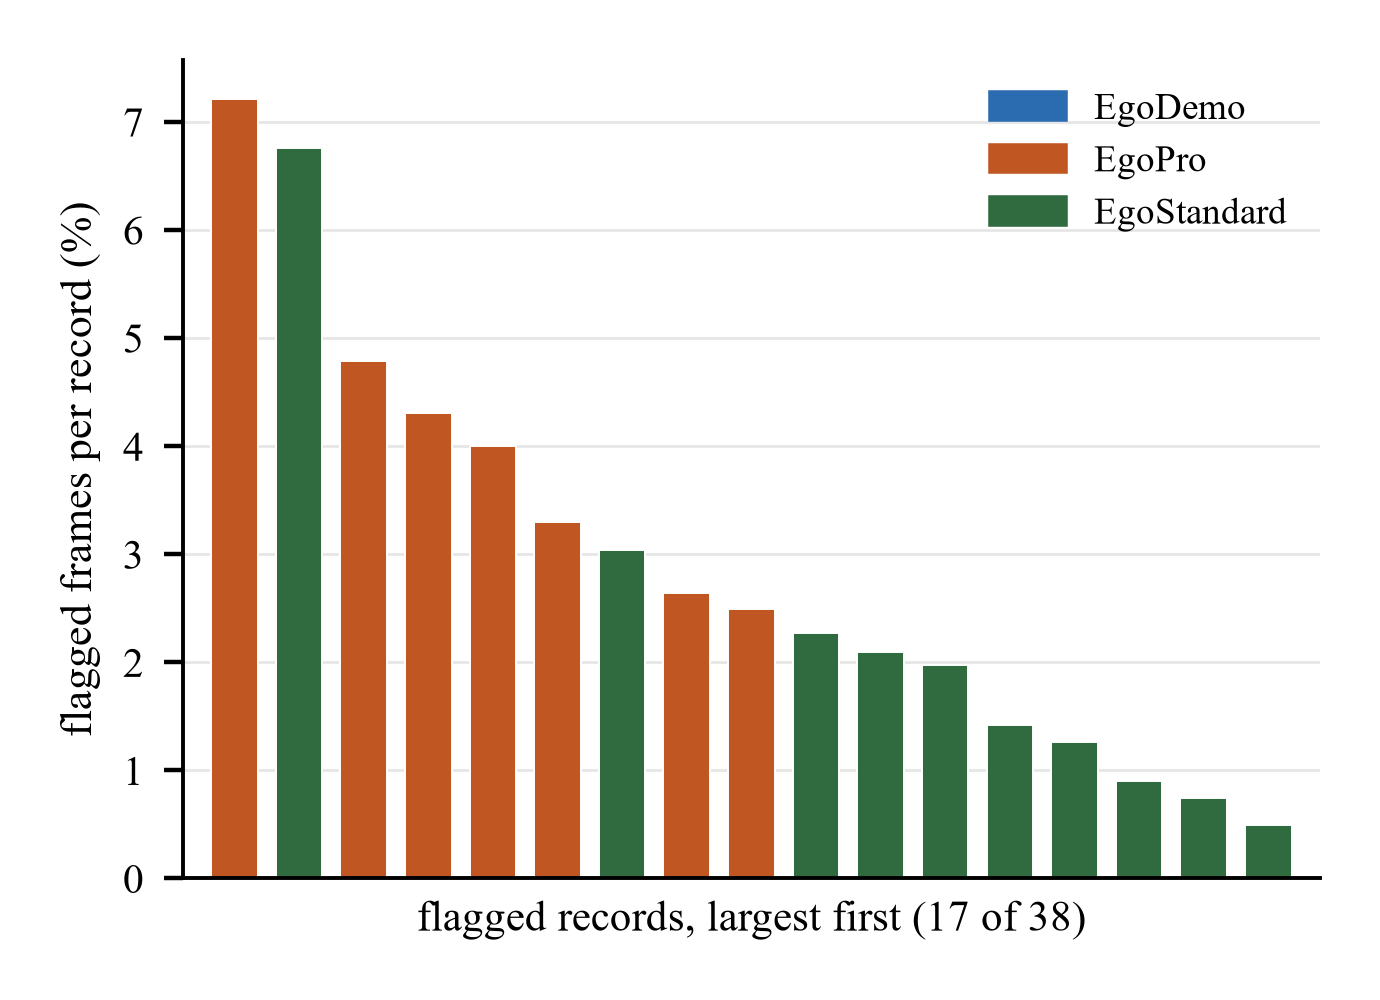
\includegraphics[width=0.47\linewidth]{figures/fig_n_badshare.png}}
\hfill
\subfigure[ARI gain of the learned decoder]{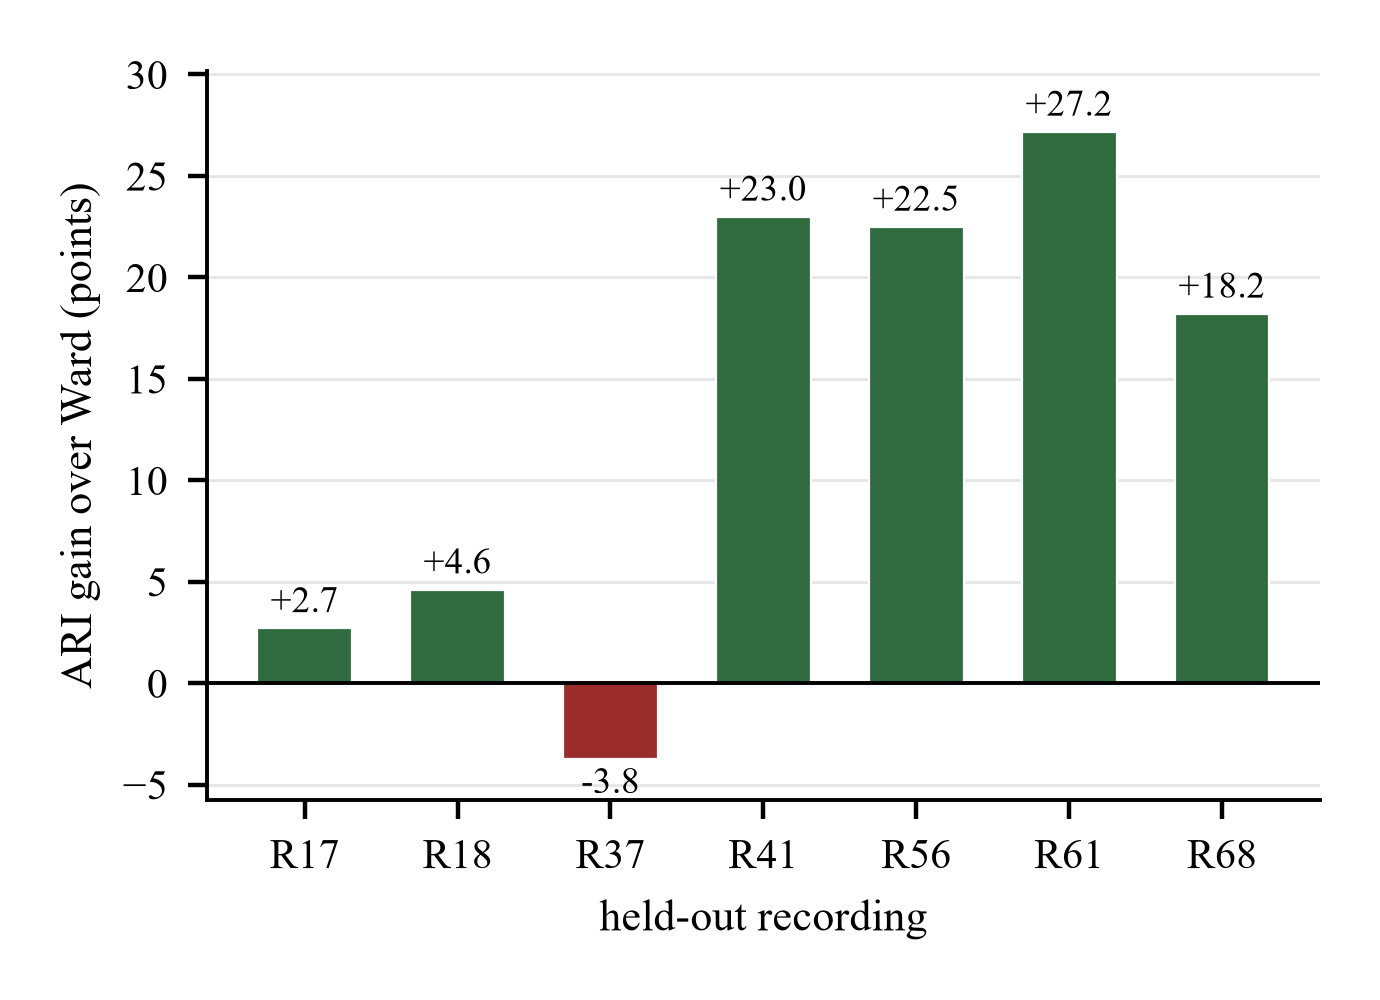
\includegraphics[width=0.47\linewidth]{figures/fig_n_arigain.png}}
\caption{Two views of the same evaluation records: the seventeen records that carry any flag
(left, ordered by share, out of the thirty-eight annotated records), and the per-record gain
of the learned boundary decoder over chain-constrained agglomeration (right), positive on six
of seven held-out records.}
\label{fig:twoviews}
\end{figure}
% numerals-ok: end
